\RussianSourceFrame{GELFAND-P001475}{70}
Гессиан — квадр. форма на пр-ве (13), инвар.
опред. в крит. точке.
\begin{equation*}
H(\varphi)=\int_M\operatorname{Tr}(\nabla_{ad}\varphi\cdot\varphi),
\qquad \varphi\in T_{X,\nabla}, \tag{14}
\end{equation*}
\begin{equation*}
\Omega^1(M)\otimes\mathrm{su}_2
\overset{\nabla_{ad}}{\longrightarrow}
\Omega^2(M)\otimes\mathrm{su}_2. \tag{15}
\end{equation*}
Если связность была интегрир., то $\nabla_{ad}$ — комплекс
([зачёркнут знак:
\RussianUnclear{GELFAND-P001475}{complex-cancel}{$\varphi$ / $\Phi$ / неразборчиво}]
$\nabla_{ad}^{2}=0$)
корректно опред. $\nabla_{ad}\varphi$ (не зависит от представителя
в факторе (13))

\underline{ф-я} [вставлено над строкой:
\RussianUnclear{GELFAND-P001475}{morse-function-insert}{$\int\nu$ / $\int v$}]
\underline{— морсовская} $\Longleftrightarrow$ $\nabla_{ad}$ не имеет
1-мерных когомологий, т.е.
\begin{equation*}
H^1(M,\text{любое предст. }\pi_1)=0 \tag{16}
\end{equation*}
[Под словами «любое предст. $\pi_1$» дописано: «или $\forall$ лок. сист.»]

Это равносильно тому, что
\begin{equation*}
M\text{ — гомологич. сфера, т.е. }H_1(X,\mathbb Z)=0 \tag{17}
\end{equation*}
\RussianUnclear{GELFAND-P001475}{homology-equivalence}{[В (17) написано $X$; утверждение о равносильности сохранено по источнику.]}

По станд. схеме надо рассм. градиентные потоки.

2 крит. точки $\longleftrightarrow$ 2 предст. $\pi_1$.

Соед. их траекторией из неинтегрир. связностей.

В окр. кривой выб. единую коорд. систему
\begin{center}
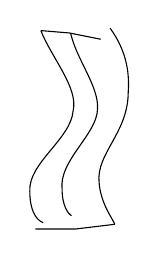
\begin{tikzpicture}[x=1cm,y=1cm]
\draw (0.04,2.50) .. controls (0.18,2.15) and (0.52,1.77) .. (0.45,1.48)
 .. controls (0.42,1.12) and (-0.12,0.82) .. (-0.10,0.46)
 .. controls (-0.10,0.23) and (-0.03,0.10) .. (0.07,0.06);
\draw (0.92,2.53) .. controls (1.11,2.27) and (1.17,2.00) .. (1.15,1.72)
 .. controls (1.15,1.20) and (0.74,0.94) .. (0.78,0.57)
 .. controls (0.80,0.31) and (0.94,0.13) .. (0.98,0.04);
\draw (0.04,2.50) -- (0.40,2.47) -- (0.80,2.39);
\draw (0.42,2.46) .. controls (0.50,2.12) and (0.78,1.79) .. (0.76,1.50)
 .. controls (0.75,1.18) and (0.27,0.85) .. (0.31,0.49)
 .. controls (0.31,0.27) and (0.39,0.17) .. (0.43,0.15);
\draw (-0.03,-0.02) -- (0.48,-0.02) -- (0.98,0.04);
\end{tikzpicture}
\end{center}
и следим за изменением матр. 2-х производных.
\begin{equation*}
\begin{aligned}
\text{Разница [вставлено: индексов]}&=
\text{числу точек [вставлено: на пути], когда возникает 0-я мода}\\
&=\text{спектр. асимметрия.}
\end{aligned}\tag{18}
\end{equation*}
Это делается с
\RussianUnclear{GELFAND-P001475}{index-theorem-cancel}{[зачёркнутое слово неразборчиво]}
пом. обычн. теор. об индексе.
\begin{equation*}
\text{Разность индексов, }\underline{\mathrm{mod}\ 8},\quad
\text{корректно определена!!} \tag{19}
\end{equation*}


\RussianSourceFrame{GELFAND-P001476}{unlabelled}
\underline{Следующий пример.}

Вычисл. индекса с точки зрения конечномерной ситуации.
(Тоже для гомологич. сферы).

\begin{center}
\begin{tikzpicture}[x=1cm,y=1cm]
\node at (0,1.4) {$N$};
\node[anchor=west] at (0.45,1.4) {— симплектич. мн-зие};
\node[rotate=-35] at (-0.50,0.68) {$\cup$};
\node[rotate=25] at (0.50,0.68) {$\cup$};
\node at (-0.95,0) {$L_1$};
\node at (0.90,0) {$L_2$};
\node[anchor=west] at (1.30,0) {— лагранжевы подмн-зия};
\node[anchor=east] at (-1.60,0.7) {(20)};
\end{tikzpicture}
\end{center}
Пусть
\begin{equation*}
L_1\cap L_2\quad\text{конечно.}\tag{21}
\end{equation*}
Хотим вычислить взвешенное число точек пересеч.

(22) \underline{Пример.} $N=$
\RussianUnclear{GELFAND-P001476}{cotangent-cancel}{[зачёркнуто: $\Omega$ / неразборчивый знак]}
$T^*L$,
\begin{center}
\begin{tikzcd}[column sep=large]
L_1=L \arrow[r,hook,"{\text{0-е сеч.}}"] & N &
L=L_2 \arrow[l,hook',"df"]
\end{tikzcd}
\end{center}
[Под $L_1=L$ зачёркнуто:
\RussianUnclear{GELFAND-P001476}{below-section-cancel}{$H_2$ / $L_2$ / неразборчиво}.]
$f$ — морсовская

$L_1\cap L_2$ — крит. точки $f$

пересеч. трансверсально.

точке пересеч. — индекс
\begin{equation*}
L_1\cap L_2\overset{\mathrm{index}}{\longrightarrow}
\{0,1,\ldots,\dim L\}
\end{equation*}
\begin{equation*}
\chi(N)=\sum_{x\in L_1\cap L_2}(-1)^{\mathrm{index}\,x}\tag{23}
\end{equation*}
\underline{Общая ситуация (20)}: опред. относительный индекс!

(24) $X$ — пути, соед. $L_1$ и $L_2$
\begin{equation*}
\begin{aligned}
[0,1]&\longrightarrow N\\
0&\longrightarrow L_1\\
1&\longrightarrow L_2
\end{aligned}
\end{equation*}
На таком $X$ есть многозначная ф-я Морса

Крит. точки — точки пересеч. $L_j$

$\varphi\in X$, $\tau$ — кас. вектор в $\varphi$, т.е. векторное поле вдоль $\varphi$

[От $\varphi$ проведена вниз короткая черта к подписи «путь».]


\RussianSourceFrame{GELFAND-P001477}{71}

Тогда
\begin{equation*}
\langle \nu,\tau\rangle := \int_0^1 \omega(\dot{\varphi},\tau),
\tag{25}
\end{equation*}
\RussianUnclear{GELFAND-P001477}{one-form-symbol}{Знак, переданный как $\nu$, может быть латинским $v$; тот же знак стоит ниже перед «морсовская».}

где

$\omega$ — симп. форма.

$\nu$ — морсовская, если $L_1$ и $L_2$ пересек. трансверсально.

Разность индексов опред., но есть и элем. конструкция

(через индекс Маслова)

Рассм. мн.-ие $M$ — гомол. сфера. !

(26) \underline{Теорема}

$M$ можно разрезать по рим. поверхности $Z$,

(разбиение Хегора)

$$
W=W_1\cup W_2,\qquad \partial W_i=Z.
$$
\RussianUnclear{GELFAND-P001477}{decomposition-letter}{В формуле написано $W$, тогда как в предшествующем тексте — $M$; отношение обозначений не пояснено.}

(27)
\begin{center}
\begin{tikzcd}[row sep=small,column sep=large]
& \pi_1(W_1) \arrow[dr] & \\
\pi_1(Z) \arrow[ur] \arrow[dr] & & \pi_1(M) \\
& \pi_1(W_2) \arrow[ur] &
\end{tikzcd}
\end{center}

общим опред. $\pi_1(M)$

$\pi_1(W_j)$ — своб. группа с $g$ образующими

Предст. $\pi_1(M)$ [зачёркнуто: \RussianUnclear{GELFAND-P001477}{cancelled-representation-word}{одно неразборчивое слово}]
— в нем $\pi_1(W_j)$ — лагранжевы мн.-ия.

Рассмотрим

(28)
\RussianSourceFigure{GELFAND-P001477}{cylinder-decomposition}{Горизонтальный рисунок: две выпуклые наружные части соединены сверху и снизу почти прямыми линиями; у соединений видны дуги, частью слабые. Над левой частью стоит $W_1$, над правой — $W_2$, под средней частью — «цилиндр». Короткие наклонные штрихи у верхних соединений не позволяют уверенно установить, являются ли они стрелками или частью контура.}

\par\medskip\noindent
\begin{minipage}[c]{0.48\linewidth}\centering
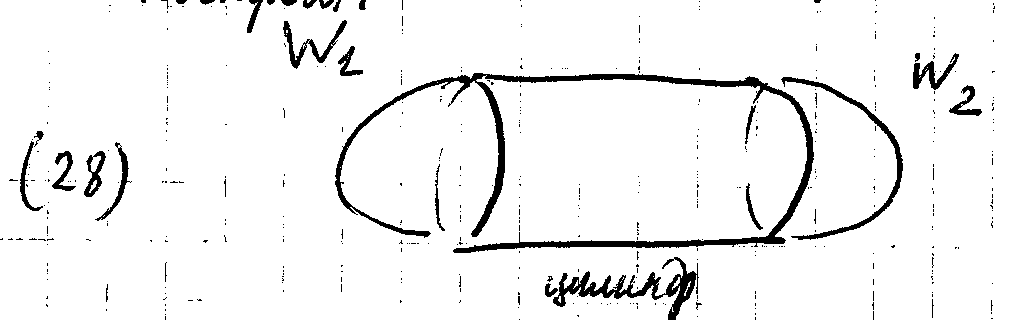
\includegraphics[width=\linewidth]{figures/gelfand-p001477-cylinder-decomposition-original.png}
\par\smallskip{\footnotesize Оригинал рукописного рисунка: GELFAND-P001477\par}
\end{minipage}\hfill
\begin{minipage}[c]{0.48\linewidth}\centering
\resizebox{\linewidth}{!}{% Partial visible-stroke recreation; uncertain connectivity remains open.
\begin{tikzpicture}[x=0.008cm,y=-0.008cm,line width=0.7pt]
\path[use as bounding box] (0,0) rectangle (1020,320);
\draw (468,78)..controls(350,76)and(282,214)..(426,233);
\draw (477,82)..controls(513,109)and(510,185)..(477,233);
\draw (446,234)..controls(431,211)and(438,178)..(437,159);
\draw (474,78)..controls(574,77)and(671,76)..(759,86);
\draw (456,248)..controls(558,242)and(667,247)..(784,239);
\draw (784,79)..controls(912,96)and(970,219)..(796,238);
\draw (765,90)..controls(827,94)and(828,193)..(778,231);
\draw (754,113)..controls(747,127)and(745,140)..(746,155);
\draw (749,187)..controls(746,208)and(754,221)..(763,228);
\draw (462,83)--(448,102);\draw (751,84)--(764,96);
\node at (320,47) {$W_1$};\node at (943,82) {$W_2$};
\node at (623,289) {цилиндр};
\end{tikzpicture}
}
\par\smallskip{\footnotesize Частичное воссоздание; неясные соединения, пересечения и наконечники остаются неустановленными.\par}
\end{minipage}\par\medskip


[зачёркнуто: \RussianUnclear{GELFAND-P001477}{cancelled-before-path}{одно неразборчивое слово перед «Путь»}]
Путь — сем-во связностей.

2-я половина раб.:

замена плоских связностей на инстантоны,

переход к $M^4$ и

инварианты Дональдсона

($M^4$ разрезается на 2 трёхмерных).
\RussianUnclear{GELFAND-P001477}{four-dimensional-cut}{Фраза «$M^4$ разрезается на 2 трёхмерных» передана буквально; размерностный смысл не уточнён.}


\RussianSourceFrame{GELFAND-P001478}{unlabelled}

\underline{12.9.88 г.}\qquad \underline{\underline{Сем. Гельфанда.}}

1. «В пр-ве какого наименьшего числа измерений две двумерные плоскости
могут скрещиваться?»

2. \underline{\underline{Что такое детерминант?}}

2 ур-я 1-го пор. можно заменить [вставлено над строкой: одним]
ур-ем 2-го порядка. Как?

\begin{equation*}
\begin{cases}
\left(\dfrac{d}{dx}+q_{11}\right)\varphi_1+q_{12}\varphi_2=0\\
q_{21}\varphi_1+\left(\dfrac{d}{dx}+q_{22}\right)\varphi_2=0
\end{cases}
\tag{1}
\end{equation*}

а) \underline{1-й способ}: выражаем из 1-го $\varphi_2$ и подст. во 2-е

\underline{2-й способ}: выражаем из 2-го $\varphi_1$ и подст. в 1-е

Получ. разные ур-я!

но решив одно, можно решить 2-е.

Это известно под назв. «преобразование Бэклунда».

Можно взять лин. комб. $\varphi_1$ и $\varphi_2$ и тогда возник. семейство ур-й.

Ответы очень красивые

б) Что для 3-х ур-й 1-го порядка?

Это уже сложнее и красота пропадает.

Сделали Гельфанд и Ретах.

Есть раб. Сато, Кашивары о некоммут. определителях.

в) Пусть $q_{ij}=\mathrm{const}$

[слева зачёркнуто: \RussianUnclear{GELFAND-P001478}{cancelled-margin-label}{неразборчивый знак пункта с правой скобкой}]
Тогда есть детерминант

\begin{equation*}
\begin{vmatrix}
\dfrac{d}{dx}+q_{11}&q_{12}\\
q_{21}&\dfrac{d}{dx}+q_{22}
\end{vmatrix}
=\left(\frac{d}{dx}\right)^2+(q_{11}+q_{22})\frac{d}{dx}
+(q_{11}q_{22}-q_{12}q_{21})
\tag{2}
\end{equation*}

$$
\frac{d}{dx}\longleftrightarrow\lambda
\qquad\Longrightarrow\qquad\text{получ. характ. опред. матрицы}
$$

в общем случае получ. [вставлено над строкой: (некоммут. аналог)]
характеристич. определителя.

$$
\begin{vmatrix}
a_{11}&a_{12}\\
a_{21}&a_{22}
\end{vmatrix}
\quad\text{— ?}
$$

$a_{ij}$ — отображение $E_j\to E_i$,

так что $a_{11}a_{22}-a_{12}a_{21}$ не имеет смысла.

Всего 4 определителя:

\begin{equation*}
a_{11}-a_{12}a_{22}^{-1}a_{21}
\tag{3}
\end{equation*}

[зачёркнуто: \RussianUnclear{GELFAND-P001478}{cancelled-final-symbol}{один знак, похожий на $a$ или «и»}]
и т.п.


\RussianSourceFrame{GELFAND-P001479}{84}

3-й порядок: 36 способов записи.

Возникает некоммут. $K$-теория и некоммут. гомологии.

\RussianUnclear{GELFAND-P001479}{overwritten-section-label}{в) / г)}
8 букв расположены кубиком $2\times2\times2$

Что такое определитель?

Это сделал Кэли.

Считалось, что после Гильберта результаты Гордана, Кэли, Клебша и др.
потеряли интерес. Они были объявлены старомодной чепухой. Но это
неверно.

\underline{\underline{Мур.}}\quad (\underline{GREGORY MOORE})\quad (\underline{I,AS. Princeton})

\underline{Конформная} \underline{теория} \underline{поля.}\quad (CFT)

Модель Изинга

\begin{center}
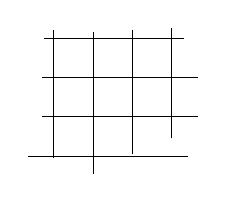
\begin{tikzpicture}[scale=0.5]
\draw (0,-0.05)--(0,3.2);
\draw (1,-0.45)--(1,3.15);
\draw (2,0.05)--(2,3.2);
\draw (3,0.45)--(3,3.25);
\draw (-0.25,3)--(3.3,3);
\draw (-0.3,2)--(3.65,2);
\draw (-0.3,1)--(3.65,1);
\draw (-0.65,0)--(3.4,0);
\end{tikzpicture}
\end{center}

2-мерн. решётка, в $\forall$ точке — переменная $\sigma :=$
[зачёркнуто: \RussianUnclear{GELFAND-P001479}{cancelled-spin-value}{короткая запись, закрытая плотными косыми штрихами}] $\pm1$

[под словом «решётка»: (квадратная)]

\begin{equation*}
\text{Энергия}\quad E=\sum_{\langle ij\rangle}\sigma_i\sigma_j
\tag{1}
\end{equation*}

$\langle ij\rangle$ — соседние точки

Статсумма

\begin{equation*}
Z=\sum e^{-\beta E}
\tag{2}
\end{equation*}

\RussianSourceFigure{GELFAND-P001479}{ising-cylinder}{Вертикальный цилиндр: замкнутый верхний овал, две боковые линии и нижняя дуга. Внутри идут несколько почти вертикальных линий; внизу видны короткий наклонный штрих слева и поперечный штрих правее. Точное соединение внутренних линий и значение коротких штрихов неясны; подписей у рисунка нет.}

\par\medskip\noindent
\begin{minipage}[c]{0.48\linewidth}\centering
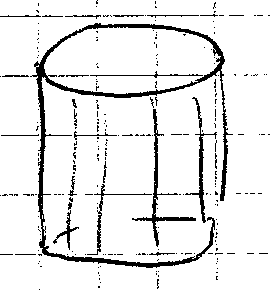
\includegraphics[width=\linewidth]{figures/gelfand-p001479-ising-cylinder-original.png}
\par\smallskip{\footnotesize Оригинал рукописного рисунка: GELFAND-P001479\par}
\end{minipage}\hfill
\begin{minipage}[c]{0.48\linewidth}\centering
\resizebox{\linewidth}{!}{% Partial visible-stroke recreation; uncertain connectivity remains open.
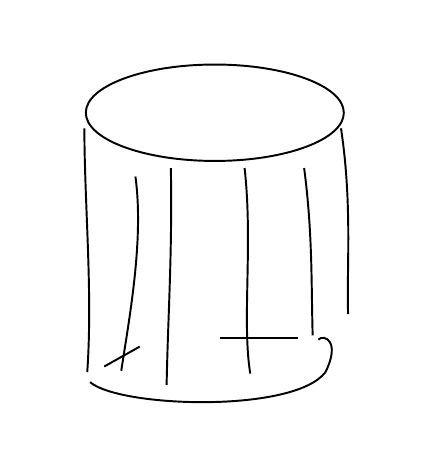
\begin{tikzpicture}[x=0.018cm,y=-0.018cm,line width=0.7pt]
\path[use as bounding box] (0,0) rectangle (270,290);
\draw (132,60) ellipse[x radius=91,y radius=34];
\draw (40,71)..controls(40,124)and(46,187)..(42,243);
\draw (221,71)..controls(229,124)and(225,168)..(226,202);
\draw (44,250)..controls(65,268)and(188,272)..(210,243);
\draw (210,243)..controls(221,221)and(209,216)..(205,220);
\draw (76,105)..controls(82,149)and(72,203)..(66,242);
\draw (101,99)..controls(102,162)and(99,201)..(98,252);
\draw (153,99)..controls(159,153)and(151,207)..(157,244);
\draw (195,99)..controls(201,145)and(200,180)..(201,217);
\draw (54,239)--(79,225);\draw (136,219)--(191,219);
\end{tikzpicture}
}
\par\smallskip{\footnotesize Частичное воссоздание; неясные соединения, пересечения и наконечники остаются неустановленными.\par}
\end{minipage}\par\medskip


Рассм. на цилиндре и измельчаем решётку

Асимптотика выраж. через ф-и

[слева зачёркнуто: \RussianUnclear{GELFAND-P001479}{cancelled-before-eta}{знак, похожий на $Z$, и следующие неразборчивые штрихи}]

$$
\eta(\tau)=q^{1/24}\prod(1-q^n),\qquad q=e^{i\pi\tau}
$$
\RussianUnclear{GELFAND-P001479}{eta-q-normalization}{В источнике $q=e^{i\pi\tau}$ вместе с $q^{1/24}\prod(1-q^n)$; согласование нормировок не уточнено.}

$$
\theta_3(\tau)=\sum e^{i\pi\tau n^2}
$$

и аналог. $\theta_2,\theta_4$

[над строкой: $\tau=i\beta$]

Инвар. относительно замены

$$
\tau\longrightarrow-1/\tau
$$

$$
Z\longrightarrow
\left|\frac{\theta_2}{\eta}\right|
+\left|\frac{\theta_3}{\eta}\right|
+\left|\frac{\theta_1}{\eta}\right|
\qquad\text{(с точн. до множителя)}
$$
\RussianUnclear{GELFAND-P001479}{last-theta-index}{Последний индекс наиболее похож на $1$; возможно $4$. Выше отдельно написано $\theta_2,\theta_4$.}

$$
Z(\beta)=Z\left(\frac{1}{\beta}\right)
$$


\RussianSourceFrame{GELFAND-P001480}{unlabelled}
In CFT we associate real analytic functions
to surfaces

\RussianSourceFigure{GELFAND-P001480}{top-torus-cycles}{Тор с отверстием; внизу дуга с подписью $\alpha$, справа поперечная дуга с подписью $\beta$. Виден наконечник влево на нижней дуге и наконечник вниз-вправо у наружного контура. Штрихи около верхнего края отверстия и разрывы поперечной дуги требуют сверки с оригиналом.}

\par\medskip\noindent
\begin{minipage}[c]{0.48\linewidth}\centering
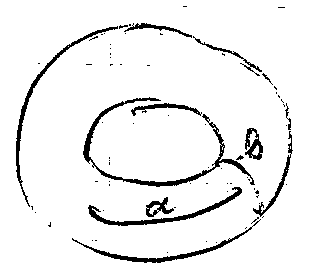
\includegraphics[width=\linewidth]{figures/gelfand-p001480-top-torus-cycles-original.png}
\par\smallskip{\footnotesize Оригинал рукописного рисунка: GELFAND-P001480\par}
\end{minipage}\hfill
\begin{minipage}[c]{0.48\linewidth}\centering
\resizebox{\linewidth}{!}{% Partial visible-stroke recreation; uncertain connectivity remains open.
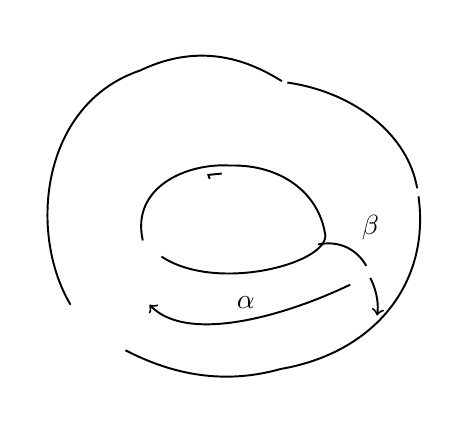
\begin{tikzpicture}[x=0.017cm,y=-0.017cm,line width=0.7pt]
\path[use as bounding box] (0,0) rectangle (310,275);
\draw (32,207)..controls(0,153)and(10,57)..(84,32)
 ..controls(130,10)and(166,25)..(190,40);
\draw (194,41)..controls(243,48)and(284,79)..(291,120);
\draw (292,126)..controls(301,191)and(259,243)..(189,255)
 ..controls(143,268)and(104,257)..(73,241);
\draw (86,159)..controls(77,119)and(119,101)..(151,103)
 ..controls(190,102)and(217,124)..(222,153)
 ..controls(229,175)and(142,199)..(100,171);
\draw (136,113)--(135,110)--(145,109);
\draw[->] (241,192)..controls(191,216)and(119,236)..(91,207);
\draw (217,162)..controls(231,159)and(245,164)..(253,178);
\draw[->] (256,187)..controls(262,199)and(262,209)..(261,215);
\node at (163,205) {$\alpha$};\node at (256,149) {$\beta$};
\end{tikzpicture}
}
\par\smallskip{\footnotesize Частичное воссоздание; неясные соединения, пересечения и наконечники остаются неустановленными.\par}
\end{minipage}\par\medskip

$$
=\sum_{i=1}^{N} f_i(\tau)\bar g_i(\tau),\qquad
f_i:=\left\{\sqrt{\frac{\theta_2}{\eta}},
\sqrt{\frac{\theta_3}{\eta}},
\sqrt{\frac{\theta_4}{\eta}}\right\}
$$
$$
\tau\to-\frac{1}{\tau},\qquad
\begin{pmatrix}f_1\\f_2\\f_3\end{pmatrix}
\to
\begin{pmatrix}0&0&1\\0&1&0\\1&0&0\end{pmatrix}
\begin{pmatrix}f_1\\f_2\\f_3\end{pmatrix}
$$

\underline{Другие варианты:}

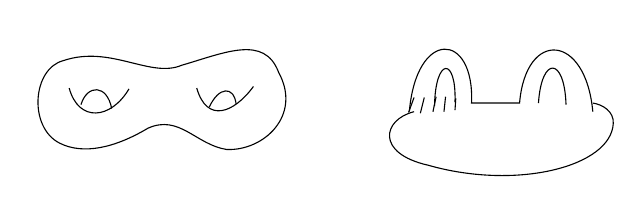
\begin{tikzpicture}[x=1cm,y=1cm]
\draw (0,0) .. controls (-.4,.2) and (-.35,.95) .. (.05,1.05)
.. controls (.65,1.25) and (1.15,.82) .. (1.55,.99)
.. controls (2.1,1.15) and (2.6,1.38) .. (2.78,.9)
.. controls (3.08,.35) and (2.59,-.1) .. (2.12,-.08)
.. controls (1.73,-.02) and (1.52,.37) .. (1.12,.19)
.. controls (.7,-.06) and (.3,-.15) .. (0,0);
\draw (.12,.7) .. controls (.24,.26) and (.65,.3) .. (.88,.69);
\draw (.27,.49) .. controls (.35,.75) and (.6,.75) .. (.66,.44);
\draw (1.74,.7) .. controls (1.87,.25) and (2.21,.38) .. (2.46,.72);
\draw (1.9,.46) .. controls (2.02,.72) and (2.21,.73) .. (2.24,.5);
\draw (4.5,.4) .. controls (4.1,.3) and (4.01,-.13) .. (4.68,-.28)
.. controls (5.8,-.6) and (7,-.3) .. (7.03,.25)
.. controls (7.04,.4) and (6.9,.49) .. (6.77,.51);
\draw (4.44,.4) .. controls (4.53,1.46) and (5.27,1.42) .. (5.23,.51)
-- (5.84,.51) .. controls (5.92,1.45) and (6.68,1.4) .. (6.77,.4);
\draw (4.76,.47) .. controls (4.77,1.1) and (5.04,1.1) .. (5.02,.52);
\draw (6.08,.51) .. controls (6.12,1.11) and (6.41,1.1) .. (6.43,.49);
\draw (4.43,.39)--(4.5,.58);
\draw (4.58,.38)--(4.63,.58);
\draw (4.74,.4)--(4.78,.59);
\draw (4.88,.4)--(4.9,.59);
\draw (5.02,.42)--(5.03,.57);
\end{tikzpicture}

На $\forall$ поверхности есть соотв. модель CFT!!

\RussianSourceFigure{GELFAND-P001480}{middle-cut-torus}{Разрезанный тор: два близких овальных торца внизу, подпись $\theta$ под разрезом, подпись $\beta$ наверху. Внутри видна изогнутая линия и плотный штрих у левого внутреннего края; различение стрелки и линии поверхности неуверенно.}

\par\medskip\noindent
\begin{minipage}[c]{0.48\linewidth}\centering
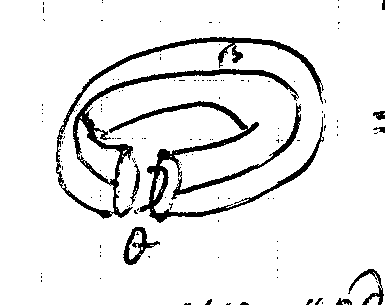
\includegraphics[width=\linewidth]{figures/gelfand-p001480-middle-cut-torus-original.png}
\par\smallskip{\footnotesize Оригинал рукописного рисунка: GELFAND-P001480\par}
\end{minipage}\hfill
\begin{minipage}[c]{0.48\linewidth}\centering
\resizebox{\linewidth}{!}{% Partial visible-stroke recreation; uncertain connectivity remains open.
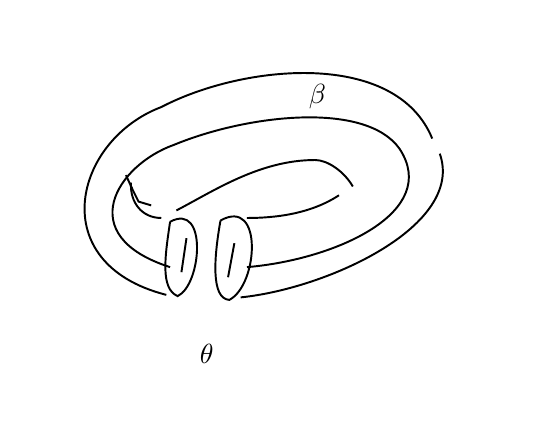
\begin{tikzpicture}[x=0.016cm,y=-0.016cm,line width=0.7pt]
\path[use as bounding box] (0,0) rectangle (385,305);
\draw (110,212)..controls(12,187)and(37,89)..(106,63)
 ..controls(171,29)and(292,17)..(321,88);
\draw (327,100)..controls(347,157)and(238,207)..(169,214);
\draw (113,190)..controls(35,165)and(71,109)..(116,93)
 ..controls(174,69)and(268,58)..(295,96)
 ..controls(328,146)and(245,184)..(174,190);
\draw (118,145)..controls(147,130)and(184,105)..(228,105)
 ..controls(238,105)and(251,114)..(258,126);
\draw (247,133)..controls(224,148)and(196,151)..(174,151);
\draw (106,151)..controls(91,151)and(81,139)..(82,123);
\draw (82,126)--(88,138)--(98,141);\draw (83,128)--(78,117);
\draw (113,154)..controls(143,138)and(138,204)..(119,213)
 ..controls(105,207)and(109,181)..(113,154);
\draw (153,153)..controls(187,134)and(183,204)..(160,216)
 ..controls(145,215)and(148,181)..(153,153);
\draw (126,167)--(122,194);\draw (164,171)--(159,198);
\node at (230,55) {$\beta$};\node at (142,259) {$\theta$};
\end{tikzpicture}
}
\par\smallskip{\footnotesize Частичное воссоздание; неясные соединения, пересечения и наконечники остаются неустановленными.\par}
\end{minipage}\par\medskip

$$
=f(\beta+i\theta,\beta-i\theta)\qquad
\text{(вещ. аналит. ф-и)}
$$
можно подкрутить по $\theta$

Параметры тора — 2 вещ. числа
$$\tau=L+i\theta$$

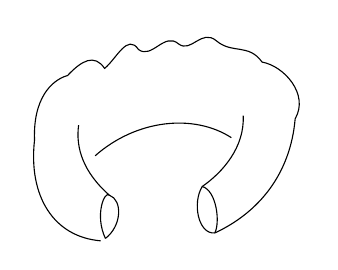
\begin{tikzpicture}[x=1cm,y=1cm]
\draw (.7,0) .. controls (.1,.05) and (-.22,.57) .. (-.14,1.28)
.. controls (-.16,1.8) and (.07,2.04) .. (.28,2.1)
.. controls (.46,2.29) and (.62,2.38) .. (.75,2.19)
.. controls (.9,2.31) and (1.04,2.64) .. (1.18,2.43)
.. controls (1.35,2.3) and (1.51,2.66) .. (1.69,2.5)
.. controls (1.85,2.38) and (1.98,2.7) .. (2.17,2.54)
.. controls (2.37,2.37) and (2.58,2.51) .. (2.75,2.27)
.. controls (3.03,2.22) and (3.35,1.86) .. (3.17,1.55)
.. controls (3.11,.85) and (2.71,.36) .. (2.15,.1);
\draw (.76,.03) .. controls (.97,.19) and (.98,.52) .. (.81,.58)
.. controls (.75,.64) and (.62,.33) .. (.76,.03);
\draw (2.15,.1) .. controls (1.94,.08) and (1.86,.48) .. (1.99,.69)
.. controls (2.17,.64) and (2.22,.24) .. (2.15,.1);
\draw (.81,.58) .. controls (.48,.87) and (.38,1.18) .. (.42,1.47);
\draw (.63,1.08) .. controls (1.15,1.54) and (1.88,1.62) .. (2.36,1.31);
\draw (1.99,.69) .. controls (2.25,.87) and (2.53,1.19) .. (2.51,1.59);
\end{tikzpicture}

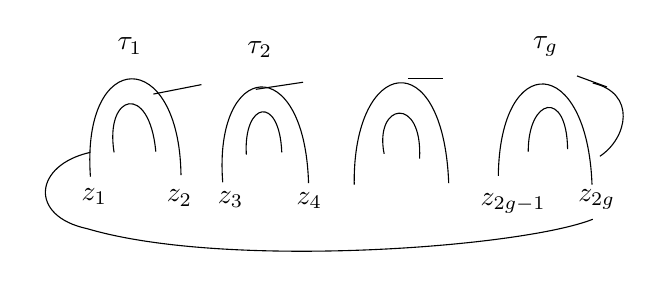
\begin{tikzpicture}[x=1cm,y=1cm]
\draw (0,.45) .. controls (-.72,.29) and (-.79,-.36) .. (-.04,-.52)
.. controls (1.72,-1.04) and (5.47,-.76) .. (6.38,-.4);
\draw (6.47,.4) .. controls (6.82,.63) and (6.94,1.2) .. (6.38,1.33);
\draw (.8,1.19)--(1.41,1.31);
\draw (2.1,1.25)--(2.7,1.34);
\draw (4.03,1.39)--(4.48,1.39);
\draw (6.18,1.42)--(6.56,1.28);
\draw (0,.14) .. controls (-.12,1.79) and (1.13,1.8) .. (1.15,.16);
\draw (.3,.45) .. controls (.18,1.2) and (.75,1.34) .. (.83,.46);
\draw (1.68,.07) .. controls (1.56,1.62) and (2.72,1.75) .. (2.77,.06);
\draw (1.98,.42) .. controls (1.94,1.09) and (2.4,1.19) .. (2.43,.45);
\draw (3.35,.04) .. controls (3.33,1.66) and (4.48,1.86) .. (4.55,.06);
\draw (3.73,.43) .. controls (3.6,1.08) and (4.22,1.18) .. (4.18,.37);
\draw (5.18,.15) .. controls (5.2,1.75) and (6.31,1.7) .. (6.37,.04);
\draw (5.56,.46) .. controls (5.56,1.14) and (6.05,1.26) .. (6.06,.49);
\node at (.5,1.8) {$\tau_1$};
\node at (2.15,1.76) {$\tau_2$};
\node at (5.78,1.79) {$\tau_g$};
\node at (.05,-.11) {$z_1$};
\node at (1.13,-.13) {$z_2$};
\node at (1.78,-.15) {$z_3$};
\node at (2.78,-.16) {$z_4$};
\node at (5.37,-.2) {$z_{2g-1}$};
\node at (6.43,-.15) {$z_{2g}$};
\end{tikzpicture}

важны длины и повороты подкрутки ручек (handles)
$$
\begin{array}{ccc}
0&1&\infty\\
\uparrow&\uparrow&\uparrow\\
z_1&z_2&z_3
\end{array}
$$
Получ. $3g-3$ компл. параметра.\qquad $(g\ge2)$
$$f(z_i,\tau_i;\bar z_i,\bar\tau_i)$$

\RussianUnclear{GELFAND-P001480}{bottom-point-pair}{$(z_{2j-1},z_{2j})$ или $(z_{j-1},z_{2j})$ или $(z_{2j+1},z_{2j})$}
— точки, в к-рые
[зачёркнуто: \RussianUnclear{GELFAND-P001480}{bottom-cancelled-word}{неразборчивое слово перед «приклеив.»}]
приклеив. ручки (тонкие)

$\tau_j$ — как в торе.


\RussianSourceFrame{GELFAND-P001481}{85}
\RussianSourceFigure{GELFAND-P001481}{top-cft-sets}{Внешний овал с надписью CFT's; внутри меньший овал с надписью RCFT's. Под ним ISING, от этой надписи вверх проходит линия, оканчивающаяся в малом овале около маленького крестика или наконечника. Точная форма последнего знака неуверенна.}

\par\medskip\noindent
\begin{minipage}[c]{0.48\linewidth}\centering
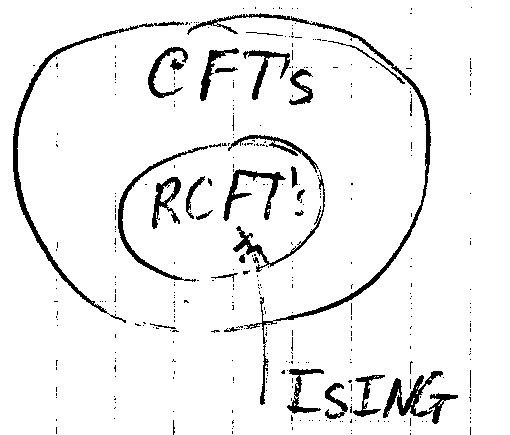
\includegraphics[width=\linewidth]{figures/gelfand-p001481-top-cft-sets-original.png}
\par\smallskip{\footnotesize Оригинал рукописного рисунка: GELFAND-P001481\par}
\end{minipage}\hfill
\begin{minipage}[c]{0.48\linewidth}\centering
\resizebox{\linewidth}{!}{% Partial visible-stroke recreation; uncertain connectivity remains open.
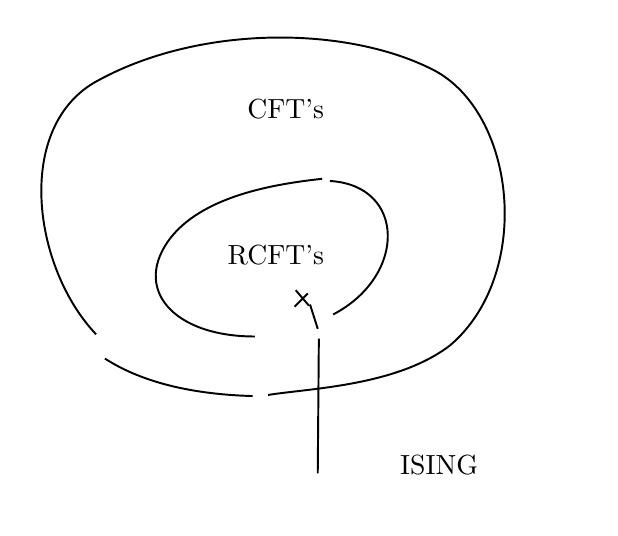
\begin{tikzpicture}[x=0.014cm,y=-0.014cm,line width=0.7pt]
\path[use as bounding box] (0,0) rectangle (510,435);
\draw (62,278)..controls(5,218)and(-12,93)..(60,50)
 ..controls(155,-4)and(293,-2)..(371,40)
 ..controls(444,82)and(457,225)..(383,288)
 ..controls(335,325)and(255,327)..(218,333);
\draw (204,334)..controls(135,332)and(95,316)..(70,300);
\draw (206,280)..controls(131,280)and(94,236)..(130,190)
 ..controls(162,150)and(232,141)..(267,137);
\draw (274,139)..controls(343,143)and(344,225)..(277,260);
\node at (234,74) {CFT's};\node at (225,206) {RCFT's};
\draw (263,404)--(264,282);\draw (263,273)--(256,251);
\draw (243,238)--(255,252);\draw (242,253)--(254,241);
\node at (373,397) {ISING};
\end{tikzpicture}
}
\par\smallskip{\footnotesize Частичное воссоздание; неясные соединения, пересечения и наконечники остаются неустановленными.\par}
\end{minipage}\par\medskip


R — Rational

I [зачёркнуто: \RussianUnclear{GELFAND-P001481}{rational-cancelled-prefix}{неразборчивые буквы после I}]
\underline{RATIONAL.}\qquad (назв. — историческое)
$$
f(z_i,\tau_i,\bar z_i,\bar\tau_i)
=\sum_{j=1}^{N<\infty}\mathcal F_j(z_i,\tau_i)
\overline{\mathcal F}_j(\bar z_i,\bar\tau_i)
$$

\underline{Тор:}
$$\theta\to\theta+2\pi$$
$$\mathcal F_j(\tau)\ne\mathcal F_j(\tau+2\pi i)$$
$$\mathcal F_j(\tau)=\sum_\ell M_{j\ell}\mathcal F_\ell(\tau+2\pi i)$$
\RussianUnclear{GELFAND-P001481}{torus-period-convention}{В обеих строках написано $\tau+2\pi i$; внизу этой страницы написано $T:\tau\to\tau+1$.}

$M=$ monodromy matrix.
[зачёркнуто: \RussianUnclear{GELFAND-P001481}{monodromy-cancelled-word}{неразборчивое слово}]

E.g. Ising
$$
Z(\tau,\bar\tau)=
\left|\sqrt{\frac{\theta_2}{\eta}}\right|^2+
\left|\sqrt{\frac{\theta_3}{\eta}}\right|^2+
\left|\sqrt{\frac{\theta_4}{\eta}}\right|^2
$$
$$\sqrt{\frac{\theta_2}{\eta}}=q^{1/8}\prod(1+q^n),\qquad q=e^{2\pi i\tau}$$
$$\sqrt{\frac{\theta_3}{\eta}}=\prod(1-q^{n-1/2})$$
$$\sqrt{\frac{\theta_4}{\eta}}=\prod(1+q^{n-1/2}).$$
\RussianUnclear{GELFAND-P001481}{ising-product-conventions}{Показатель $1/8$, знак минус в строке $\theta_3$ и знак плюс в строке $\theta_4$ воспроизведены по источнику; нормировка не уточнена.}

\underline{И.М.Г.} Эллиптич. ф-и — это тригонометрия с параметром $q$.

$\mathcal F_j$ — не инвариантны, но $f$ уже инвариантно

($\overline{\mathcal F}_j$
не обязательно компл. сопряжены к $\mathcal F_j$!)

Возникает группа кос.

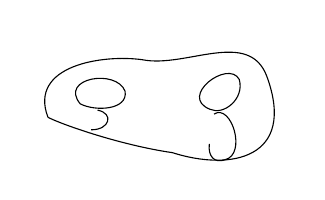
\begin{tikzpicture}[x=1cm,y=1cm]
\draw (0,.4) .. controls (-.25,1.06) and (.7,1.2) .. (1.2,1.13)
.. controls (1.75,1.02) and (2.55,1.53) .. (2.78,.92)
.. controls (3.16,-.12) and (2.33,-.29) .. (1.58,-.05)
.. controls (.89,.05) and (.12,.33) .. (0,.4);
\draw (.41,.57) .. controls (.14,.9) and (.87,1.02) .. (.98,.73)
.. controls (1.02,.49) and (.6,.47) .. (.41,.57);
\draw (2.06,.5) .. controls (1.65,.66) and (2.29,1.14) .. (2.43,.88)
.. controls (2.5,.63) and (2.23,.42) .. (2.06,.5);
\draw (.63,.49) .. controls (.84,.45) and (.79,.24) .. (.55,.24);
\draw (2.11,.44) .. controls (2.33,.58) and (2.53,-.07) .. (2.25,-.14)
.. controls (2.12,-.19) and (2.03,-.1) .. (2.05,.06);
\end{tikzpicture}

Generalize.

$g=1$
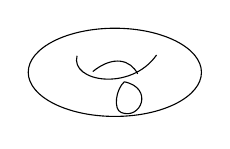
\begin{tikzpicture}[x=1cm,y=1cm]
\draw (0,0) ellipse (1.1cm and .56cm);
\draw (-.48,.21) .. controls (-.57,-.12) and (.2,-.25) .. (.53,.22);
\draw (-.28,.01) .. controls (-.02,.22) and (.2,.16) .. (.29,-.02);
\draw (.12,-.12) .. controls (.5,-.2) and (.33,-.61) .. (.08,-.51)
.. controls (-.02,-.47) and (.01,-.22) .. (.12,-.12);
\end{tikzpicture}
$$
S:\tau\to-1/\tau\qquad
T:\tau\to\tau+1
$$
$$S^2=1,\qquad (ST)^3=I$$


\RussianSourceFrame{GELFAND-P001482}{unlabelled}
\underline{``DEHNTWIST''}

\underline{$g=2$}
\RussianSourceFigure{GELFAND-P001482}{top-genus-two-twists}{Двуручная поверхность с кривыми и подписями $\alpha_1,\beta_1$ у левой ручки, $\alpha_2$ вдоль средней части и $\beta_2,\alpha_3$ у правой ручки. Часть кривых перекрывает края отверстий; разрывы и соединения штрихов не позволяют уверенно восстановить все прохождения.}

\par\medskip\noindent
\begin{minipage}[c]{0.48\linewidth}\centering
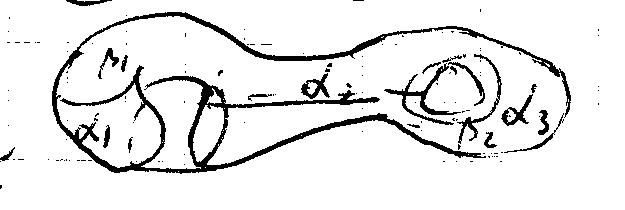
\includegraphics[width=\linewidth]{figures/gelfand-p001482-top-genus-two-twists-original.png}
\par\smallskip{\footnotesize Оригинал рукописного рисунка: GELFAND-P001482\par}
\end{minipage}\hfill
\begin{minipage}[c]{0.48\linewidth}\centering
\resizebox{\linewidth}{!}{% Partial visible-stroke recreation; uncertain connectivity remains open.
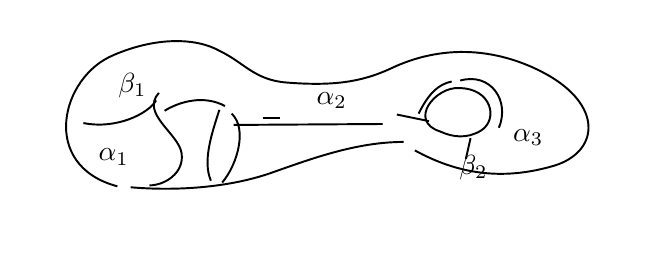
\begin{tikzpicture}[x=0.012cm,y=-0.012cm,line width=0.7pt]
\path[use as bounding box] (0,0) rectangle (625,210);
\draw (95,168)..controls(12,146)and(35,52)..(91,29)
 ..controls(135,10)and(178,10)..(204,25)
 ..controls(229,37)and(240,55)..(273,58)
 ..controls(322,62)and(353,58)..(385,43)
 ..controls(453,11)and(515,29)..(554,52)
 ..controls(610,86)and(603,132)..(558,146)
 ..controls(501,163)and(454,154)..(410,130);
\draw (398,121)..controls(348,121)and(300,139)..(260,153)
 ..controls(213,170)and(155,173)..(109,169);
\draw (145,88)..controls(161,78)and(187,71)..(209,83);
\draw (216,91)..controls(233,107)and(222,145)..(206,164);
\draw (139,69)..controls(119,91)and(160,112)..(163,133)
 ..controls(166,154)and(145,167)..(129,167);
\draw (203,87)..controls(195,112)and(185,141)..(194,162);
\draw (59,101)..controls(94,108)and(128,91)..(136,77);
\draw (218,103)--(376,102);\draw (249,96)--(267,96);
\draw (437,110)..controls(402,99)and(432,62)..(457,64)
 ..controls(491,64)and(499,97)..(480,109)
 ..controls(465,118)and(450,116)..(437,110);
\draw (414,91)..controls(425,69)and(435,60)..(449,57);
\draw (458,56)..controls(490,47)and(511,77)..(499,106);
\draw (391,92)--(425,99);\draw (469,117)--(464,139);
\node at (91,137) {$\alpha_1$};\node at (111,61) {$\beta_1$};
\node at (322,77) {$\alpha_2$};\node at (472,148) {$\beta_2$};
\node at (530,116) {$\alpha_3$};
\end{tikzpicture}
}
\par\smallskip{\footnotesize Частичное воссоздание; неясные соединения, пересечения и наконечники остаются неустановленными.\par}
\end{minipage}\par\medskip

$$z_i,\tau_i\to\tilde z_i,\tilde\tau_i$$

$$\alpha_1\beta_1\alpha_1=\beta_1\alpha_1\beta_1$$
$$\alpha_2\beta_2\alpha_2=\beta_2\alpha_2\beta_2$$
$$\alpha_2\beta_1\alpha_2=\beta_1\alpha_2\beta_1\qquad(\beta_1\to\beta_2)$$
$$\alpha_1\alpha_2=\alpha_2\alpha_1$$
$$\beta_1\beta_2=\beta_2\beta_1\qquad\text{etc.}$$
$$ (\alpha_1\beta_1\alpha_2)^4=\alpha_3^2 $$
$$ (\alpha_3\beta_2\alpha_2\beta_1\alpha_1^2\beta_1\alpha_2\beta_2\alpha_3)^2=1 $$
$$ \beta_1^{-1}\alpha_1\beta_1=\alpha_1\beta_1\alpha_1^{-1}. $$

[Две горизонтальные черты с точкой между ними.]

CFT.
$$\mathcal A=\{(\sigma,\Delta)\ \text{fields}\}=\text{operator algebra}$$
$$\mathcal A\qquad\{T(z),T'(z),\ldots\}$$
$$
\mathcal H=\bigoplus_{i=1}^{N}
\underset{\mathcal A}{\mathcal H_i}\otimes
\underset{\bar{\mathcal A}}{\mathcal H_{\bar i}}
$$
$$\Delta:\mathcal A\to\mathcal A\otimes\mathcal A$$
$$ L_n=\oint_c\zeta^{n+1}T(\zeta) $$
$$ \to\oint\zeta^{n+1}T(\zeta)\otimes1+1\otimes\oint\zeta^{n+1}T(\zeta) $$
\RussianUnclear{GELFAND-P001482}{ln-integration-symbol}{Буква переменной похожа на $\zeta$ или $\xi$; под первым контурным интегралом $c$ или $C$. Дифференциал в этих строках не написан.}

$\rho_i:\mathcal A\to\operatorname{End}\mathcal H_i$,\qquad
\RussianUnclear{GELFAND-P001482}{rho-trailing-fragment}{$\rho_i\,C$ или $\rho_i\,O$; короткий фрагмент без видимого продолжения}

[Разделительная строка из мелких штрихов.]

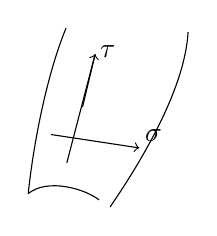
\begin{tikzpicture}[x=1cm,y=1cm]
\draw (0,0) .. controls (.08,.76) and (.27,1.6) .. (.48,2.1);
\draw (1.04,-.17) .. controls (1.49,.49) and (1.99,1.36) .. (2.03,2.05);
\draw (0,0) .. controls (.25,.2) and (.72,.06) .. (.9,-.08);
\draw (.49,.39)--(.85,1.77);
\draw[->] (.69,1.1)--(.85,1.77);
\draw[->] (.29,.75)--(1.41,.58);
\node at (1.01,1.8) {$\tau$};
\node at (1.59,.74) {$\sigma$};
\end{tikzpicture}
$$
S=\int g_{\mu\nu}(X)
[(\partial_\sigma X^\mu)(\partial_\sigma X^\nu)
-(\partial_\tau X^\mu)(\partial_\tau X^\nu)]
$$
Conformal Invariance $\to R_{\mu\nu}=0$.


\RussianSourceFrame{GELFAND-P001483}{86}

\underline{И.М.Г.} Что должно заменить понятие пр-ва при квантовании?

(планковская длина есть $\sim 10^{-33}$ м)
\RussianUnclear{GELFAND-P001483}{planck-unit}{Единица после $10^{-33}$: м.}

\underline{1 вар.}: нечто дискретное.

Риман понимал, что это важно, и продумывал понятие пр-ва.

Тонкая пленка около 4-мерной поверхности.

\underline{Разумное упр.}: наивная геометрия 4-мерных многогранников.

\begin{center}
\begin{tikzpicture}[x=1cm,y=1cm]
\draw (0,0) -- (0.75,-0.03);
\draw (1.07,0.01) -- (1.04,-0.12);
\draw (1.43,0.01) -- (2.47,-0.04);
\end{tikzpicture}
\end{center}

$$
S=\int_{R^4}g_{\mu\nu}(X)
\bigl[(\partial_\sigma X^\mu)(\partial_\sigma X^\nu)
-(\partial_\tau X^\mu)(\partial_\tau X^\nu)\bigr]+S_K
$$

[Под интегральным членом фигурная скобка; под ней и справа:]
$$
\begin{array}{ccc}
c_{R^4}&+c_K=&26\\
\Vert&&\\
4&&
\end{array}
$$

[От $S_K$ короткая черта к помете:]
компактный
\RussianUnclear{GELFAND-P001483}{sk-annotation}{конд. на утолщ. пр-ва / конд. на уплотн. пр-ва / конд. на уполщ. пр-ва / конд. на уплощ. пр-ва}

можно заменить на $\forall$ другую модель с нек-рыми
св-вами инвариантности

$$
c\left(\begin{gathered}\text{conformal Field}\\\text{Theory}\end{gathered}\right)\text{ — }?
$$

[Под «Theory» короткая вертикальная черта и помета «любая»;
к «любая» снизу проведена фигурная линия от пометы слева «тоже им. смысл.».]

Поэтому [зачеркнуто:
\RussianUnclear{GELFAND-P001483}{cft-cancellation}{имеет / имеют}]
это интересно.

\underline{19.9.88 г.}\qquad\underline{Сем. Гельфанда.}

\underline{\underline{Морозов А.}}

\underline{Конформная теория поля}
(по мотивам докл. Мура).

Теория струн развивается с 1984 года.

\underline{Исходная картинка}

\begin{center}
\begin{tikzpicture}[x=1cm,y=1cm]
\draw (0,2.14) .. controls (0.24,2.25) and (0.32,1.97) .. (0.21,1.91)
 .. controls (0.03,1.80) and (0.37,1.71) .. (0.27,1.50);
\fill (0,2.14) circle (0.04);
\fill (0.27,1.50) circle (0.055);
\node[anchor=west] at (1.40,1.85) {в $R^{26}$};
\node[anchor=west] at (4.25,1.85) {$x^\beta,\quad\varphi(x)$ — поле};
\node[anchor=west] at (-0.05,0.83) {$x^\mu(\sigma)$};
\node[anchor=west] at (3.05,0.66) {$\Phi\{x_\mu(\sigma)\}$};
\node[anchor=west] at (6.25,0.66) {$\mu=1,\ldots,26$};
\node[anchor=west] at (-0.05,-0.23) {$\Phi\{C\}$};
\draw[->] (2.85,0.48) -- (1.60,-0.06);
\node[anchor=west] at (1.80,-0.35) {— ф-л от};
\end{tikzpicture}
\end{center}

\RussianUnclear{GELFAND-P001483}{field-overwrite}{В строке «поле» знак перед $(x)$ переписан: $\varphi$ / $\Phi$.}
\RussianUnclear{GELFAND-P001483}{contour-ending}{После «ф-л от»: контура / контуров; конец слова переписан.}

\begin{equation*}
(1)\quad
\langle\varphi(x_1)\ldots\varphi(x_n)\rangle
=\int D\varphi\,e^{\Sigma(\varphi)}\varphi(x_1)\ldots\varphi(x_n)
\end{equation*}

\RussianUnclear{GELFAND-P001483}{eq1-first-symbol}{Первый знак поля в (1) переписан: $\varphi$ / $\Phi$.}

\RussianSourceFigure{GELFAND-P001483}{particle-diagram}{Три линии с подписями $x_1$, $x_2$, $x_3$ слева. Верхняя линия волнистая; средняя и нижняя поднимаются вправо к двум местам на верхней линии. В первом месте темная точка; справа темная точка или наконечник. Точные соединения штрихов в этих местах неясны.}

\par\medskip\noindent
\begin{minipage}[c]{0.48\linewidth}\centering
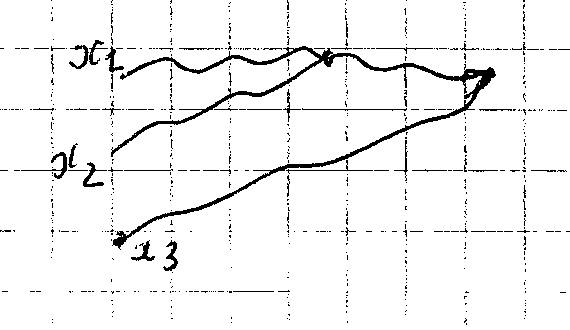
\includegraphics[width=\linewidth]{figures/gelfand-p001483-particle-diagram-original.png}
\par\smallskip{\footnotesize Оригинал рукописного рисунка: GELFAND-P001483\par}
\end{minipage}\hfill
\begin{minipage}[c]{0.48\linewidth}\centering
\resizebox{\linewidth}{!}{% Partial visible-stroke recreation; uncertain connectivity remains open.
\begin{tikzpicture}[x=0.014cm,y=-0.014cm,line width=0.7pt]
\path[use as bounding box] (0,0) rectangle (570,330);
\draw (126,78)..controls(161,55)and(166,52)..(187,66)
 ..controls(207,79)and(227,48)..(245,59)
 ..controls(265,72)and(287,46)..(302,48);
\draw (309,51)..controls(319,58)and(327,64)..(336,61)
 ..controls(367,56)and(370,78)..(395,69)
 ..controls(421,57)and(452,77)..(463,77);
\draw (117,151)..controls(157,124)and(182,126)..(198,120)
 ..controls(230,113)and(243,89)..(260,94)
 ..controls(286,104)and(302,81)..(321,65);
\draw (122,238)..controls(158,207)and(189,214)..(219,195)
 ..controls(253,176)and(278,165)..(305,166)
 ..controls(340,166)and(393,132)..(429,123)
 ..controls(457,117)and(471,98)..(480,82);
\draw[line width=1.3pt] (319,63)--(329,55);\draw[line width=1.3pt] (470,78)--(489,72);
\node at (90,49) {$x_1$};\node at (70,162) {$x_2$};\node at (157,260) {$x_3$};
\end{tikzpicture}
}
\par\smallskip{\footnotesize Частичное воссоздание; неясные соединения, пересечения и наконечники остаются неустановленными.\par}
\end{minipage}\par\medskip


(Вначале было 3 частицы, в конце ничего не осталось)

$\Sigma(\varphi)$ наз. квантовое действие


\RussianSourceFrame{GELFAND-P001484}{unlabelled}

Хотим то же в теор. струн

\begin{equation*}
(2)\quad
\langle\Phi(C_1)\ldots\Phi(C_n)\rangle
\longrightarrow
\int D\Phi\,e^{\Sigma(\Phi)}\Phi(C_1)\ldots\Phi(C_n);
\end{equation*}

\RussianUnclear{GELFAND-P001484}{eq2-relation}{Переписанный знак перед интегралом: $\longrightarrow$ / $\Rightarrow$ / $=$.}

но в этом напр. никакого разумного прогресса нет!

Но: левую часть (2) можно опис. в других терминах.

\begin{equation*}
(3)\quad
\Phi(C)=\sum\varphi_n(x)e^{in\sigma}\qquad(\text{замкн. струна})
\end{equation*}

$\varphi_n$ — отожд. с полями в (1)

Рассмотрим

\begin{equation*}
(4)\quad
\langle\varphi_{N_1}(x_1)\ldots\varphi_{N_n}(x_n)\rangle
\end{equation*}

и для нее пишем другое предст.

\begin{equation*}
(5)\quad
\langle\varphi(x_1)\varphi(x_2)\rangle
=\int Dx\,e^{-mL},\qquad
L=\int\sqrt{\dot{x}^2}\,dt
\end{equation*}

\RussianUnclear{GELFAND-P001484}{eq5-exponent-overwrite}{В показателе экспоненты буква после минуса переписана; видимое чтение $-mL$, первоначальные штрихи неразборчивы.}

[Под левой частью (5) вертикально поставленный знак равенства:]
$$
\begin{gathered}
\Vert\\
\int D\varphi\,e^{\Sigma_0(\varphi)}\varphi(x_1)\varphi(x_2)
\end{gathered}
$$

для [вставлено сверху: простейшего] действия $\Sigma_0$, опис. своб. частицу.

\begin{equation*}
(6)\quad
\Sigma_0(\varphi)=\int(\partial\varphi)^2\partial^{26}x
+\int\varphi^3d^{26}x
\end{equation*}

\RussianUnclear{GELFAND-P001484}{eq6-measure}{Первый знак меры: $\partial$.}
\RussianUnclear{GELFAND-P001484}{eq6-cubic-free}{Второе слагаемое: $+\int\varphi^3d^{26}x$.}

Теперь

\begin{equation*}
(7)\quad
\langle\varphi_{N_1}(x_1)\ldots\varphi_{N_n}(x_n)\rangle
\sim\int Dx\,e^S\,V_{N_1}(x)\ldots V_{N_n}(x),
\end{equation*}

[Под интегралом:]
по мир. поверхн. $x^\mu(\sigma,t)$
(несингулярным) и по всем топологиям

$V_{N_j}$ — вершинные операторы
\RussianUnclear{GELFAND-P001484}{vertex-index}{Маленький нижний индекс при $N$: $j$ / $d$.}

(8)
\RussianSourceFigure{GELFAND-P001484}{branching-diagram}{Лентовидная фигура: слева почти вертикальный край, сверху и снизу изогнутые границы до второй почти вертикальной черты. Справа расходятся четыре кривые; две внутренние пересекаются. Точное сопряжение границ со второй вертикальной чертой и значение пересечения неясны. Справа из области слова «ветвления» идет большая изогнутая стрелка влево к рисунку.}

\par\medskip\noindent
\begin{minipage}[c]{0.48\linewidth}\centering
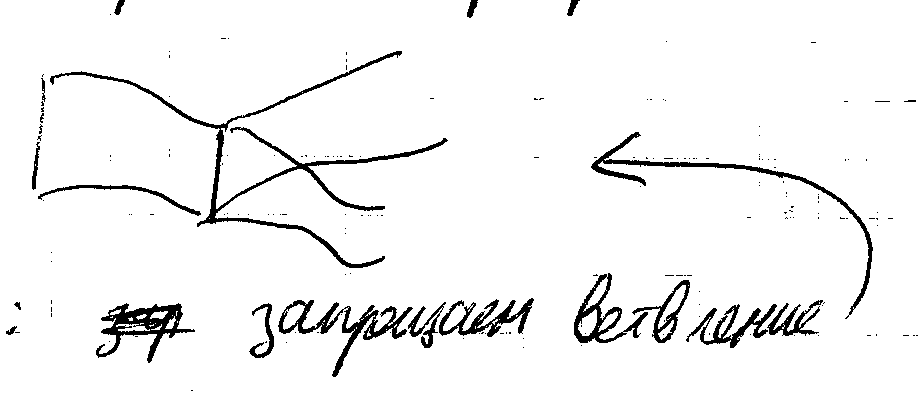
\includegraphics[width=\linewidth]{figures/gelfand-p001484-branching-diagram-original.png}
\par\smallskip{\footnotesize Оригинал рукописного рисунка: GELFAND-P001484\par}
\end{minipage}\hfill
\begin{minipage}[c]{0.48\linewidth}\centering
\resizebox{\linewidth}{!}{% Partial visible-stroke recreation; uncertain connectivity remains open.
\begin{tikzpicture}[x=0.009cm,y=-0.009cm,line width=0.7pt]
\path[use as bounding box] (0,0) rectangle (920,400);
\draw (42,80)--(34,187);
\draw (52,78)..controls(119,53)and(167,110)..(216,123);
\draw (41,198)..controls(110,169)and(156,193)..(199,213);
\draw (221,135)--(210,214);
\draw (230,123)..controls(288,111)and(337,74)..(399,55);
\draw (233,130)..controls(281,140)and(301,171)..(321,191)
 ..controls(342,213)and(365,210)..(383,209);
\draw (220,208)..controls(248,183)and(281,170)..(302,166)
 ..controls(355,158)and(424,162)..(445,142);
\draw (218,222)..controls(271,219)and(303,221)..(326,245)
 ..controls(340,265)and(361,275)..(381,259);
\draw[->] (845,343)..controls(935,184)and(806,165)..(593,167);
\draw (593,167)--(636,133);\draw (593,167)--(644,186);
\node at (522,326) {запрещены ветвления};
\end{tikzpicture}
}
\par\smallskip{\footnotesize Частичное воссоздание; неясные соединения, пересечения и наконечники остаются неустановленными.\par}
\end{minipage}\par\medskip


Теор. струн: [зачеркнуто:
\RussianUnclear{GELFAND-P001484}{branching-cancellation}{зап / запр}]
запрещены ветвления

\begin{center}
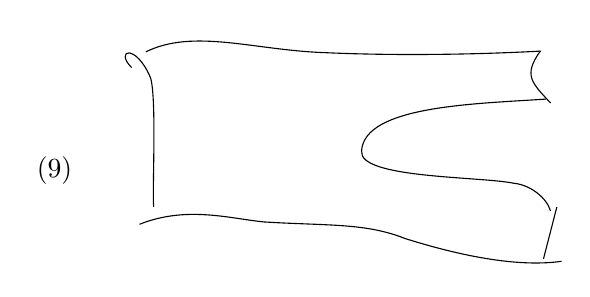
\begin{tikzpicture}[x=1cm,y=1cm]
\node[anchor=east] at (-0.55,1.12) {(9)};
\draw (0.26,2.63) .. controls (0.87,2.93) and (1.64,2.65) .. (2.53,2.62)
 .. controls (3.63,2.57) and (4.75,2.61) .. (5.28,2.64);
\draw (0.08,2.43) .. controls (-0.14,2.65) and (0.13,2.75) .. (0.32,2.30)
 .. controls (0.40,2.04) and (0.34,0.85) .. (0.36,0.66);
\draw (5.27,2.64) .. controls (5.05,2.33) and (5.16,2.24) .. (5.40,1.98);
\draw (5.34,2.03) .. controls (4.47,1.97) and (3.03,1.95) .. (3.00,1.37)
 .. controls (2.96,1.02) and (4.51,1.05) .. (4.94,0.96)
 .. controls (5.14,0.94) and (5.35,0.78) .. (5.40,0.61);
\draw (5.48,0.66) -- (5.31,0.00);
\draw (0.18,0.44) .. controls (0.78,0.68) and (1.34,0.51) .. (1.76,0.47)
 .. controls (2.56,0.42) and (3.05,0.46) .. (3.55,0.26)
 .. controls (4.09,0.09) and (4.91,-0.12) .. (5.54,-0.03);
\end{tikzpicture}
\end{center}

(но такие превращ. остаются!)

и получается теория своб. частиц.

